\chapter{Introduction}

\section{}{Présentation de l'entreprise d'accueil}
Créée en 2003 par Laurent Py et Bruno LEGEARD, la société LEIROS est spécialisée dans le test logiciel. Elle est issue du projet Smart Testing\texttrademark ~au LIFC\footnote{Laboratoire d'informatique de Franche-Comté}. L'objectif premier de LEIROS a été d'industrialiser le projet Smart Testing\texttrademark.  LEIROS a ensuite changé de nom pour devenir SMARTESTING en juin 2008. En septembre 2008, Smartesting ouvre sa filiale à Bangalore, en Inde. SMARTESTING compte environ trente-cinq personnes dont onze dans le service R\&D{}\footnote{Recherche et développement}.

\subparagraph*{}
Smartesting est implantée dans différents points stratégiques. En France,le siège social ainsi que le centre R\&D sont à Besançon dans les locaux de l'hôtel d'entreprises TEMIS Innovation. Ainsi la R\&D reste proche géographiquement de l'université et de la recherche qui y a lieu. À Paris et à Amsterdam aux Pays-Bas se trouvent les agences où travaillent les commerciaux et les avant-vente. Smartesting s'est implantée à Bangalore, en Inde où elle compte réaliser la moitié de son chiffre d'affaires en 2010 grâce au boom de l'offshore où le marché du test logiciel est en pleine expansion.

%TODO : figure de temis innovation



\subparagraph*{}
Smartesting développe dans le secteur grandissant du test logiciel. Ce marché devrait atteindre 13 milliards de dollars en 2010 (selon une étude de Gartner). Le test logiciel, en particulier le test fonctionnel devient une phase clé du développement logiciel. Des besoins très stricts pour les milieux bancaires par exemple obligent ces entreprises à faire appel à des ingénieurs et des architectes de test afin de concevoir les tests logiciels qui permettront par exemple de garantir la stabilité, la non regression et le bon fonctionnement de gros projets. SMARTESTING propose Test Designer, une solution de génération automatique de référentiels de test à plusieurs niveaux.

\subparagraph*{}
L'entreprise est organisée autour d'un directoire de trois personnes : Laurent PY, Bruno LEGEARD et Stéphane WERBA.Je travaille dans le service de R\&D{}\ de SMARTESTING.  L'équipe est composée de 11 ingénieurs dévelopeurs qui améliorent sans cesse le produit Test Designer ainsi que les connecteurs et les publishers y sont développés. L'équipe fonctionne autour de méthodes Agiles, en particulier eXtreme Programming. Ces sujets seront développés dans les sections qui vont suivre.

\begin{figure}[!h]
\centering
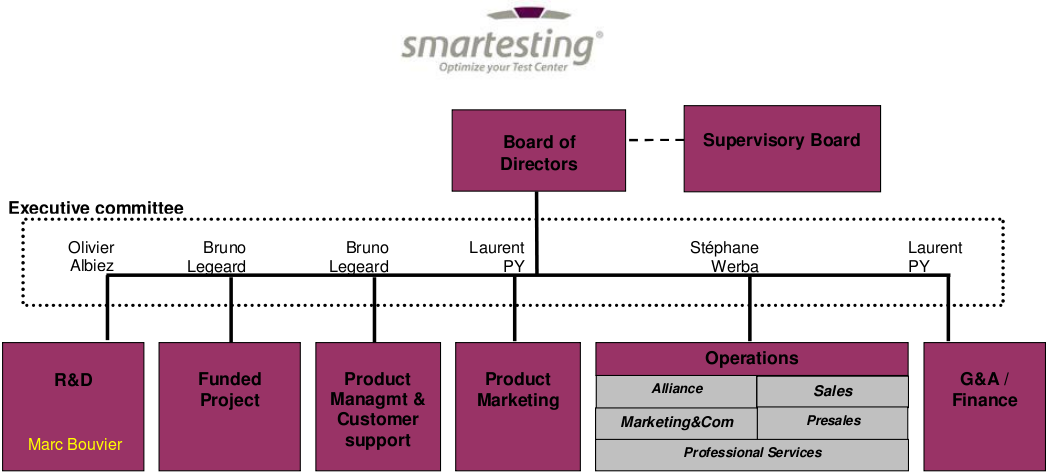
\includegraphics[scale=0.50]{Illustrations/Organigramme_with_me.png}
\caption{Organigramme}
\label{fig:Organigramme de Smartesting}
\end{figure}

\section{Test Designer}
La solution Test Designer permet de générer des référentiels de tests fonctionnels à partir de modèles UML pour le test/footnote{Model Based Testing}. Elle s'appuie sur des modeleurs UML basés sur Eclipse\footnote{Eclipse est une plateforme applicative sur laquelle peuvent se greffer des applications clientes sous forme de plugins(extensions)} 
\section{Methodes Agiles}
TODO : déroulement d'un semaine "agile"
Méthode Agile : eXtreme Programming  (XP)
Les méthodes Agiles et l'eXtreme Programming sont un ensemble de bonne pratiques dédiées à la production logicielle. Elles ont comme philosophie accepter le changement plutôt que de le supporter. L'eXtreme Programming (XP) pr\^one les cycles de développement courts (1 à 2 semaines). Un Client XP\footnote{Client sur site interne} permet d'avoir des retours rapides et de s'assurer que les exigences fonctionnelles soient bien comprises et implémentées.

L'eXtreme Programming repose sur cinq valeurs
\begin{itemize}
\item{La communication}
\item{La simplicité}
\item{Le feedback}
\item{Le courage}
\item{Le respect}
\end{itemize}
\subsection{Itération}
L'équipe organise son travail sous forme d'itération, chaque itération traite un nombre de fonctionnalités limité quantifié sous forme de points de vélocité. Une itération est planifiée lors de la rétrospective de l'itération précédente. Un itération compte un certain nombre de points de vélocité qui est en fait un objectif à atteindre par l'équipe de développement. La durée d'une itération est en général inférieure à 2 semaines. A la fin d'une itération le produit est livré.
\begin{figure}[!h]
\centering
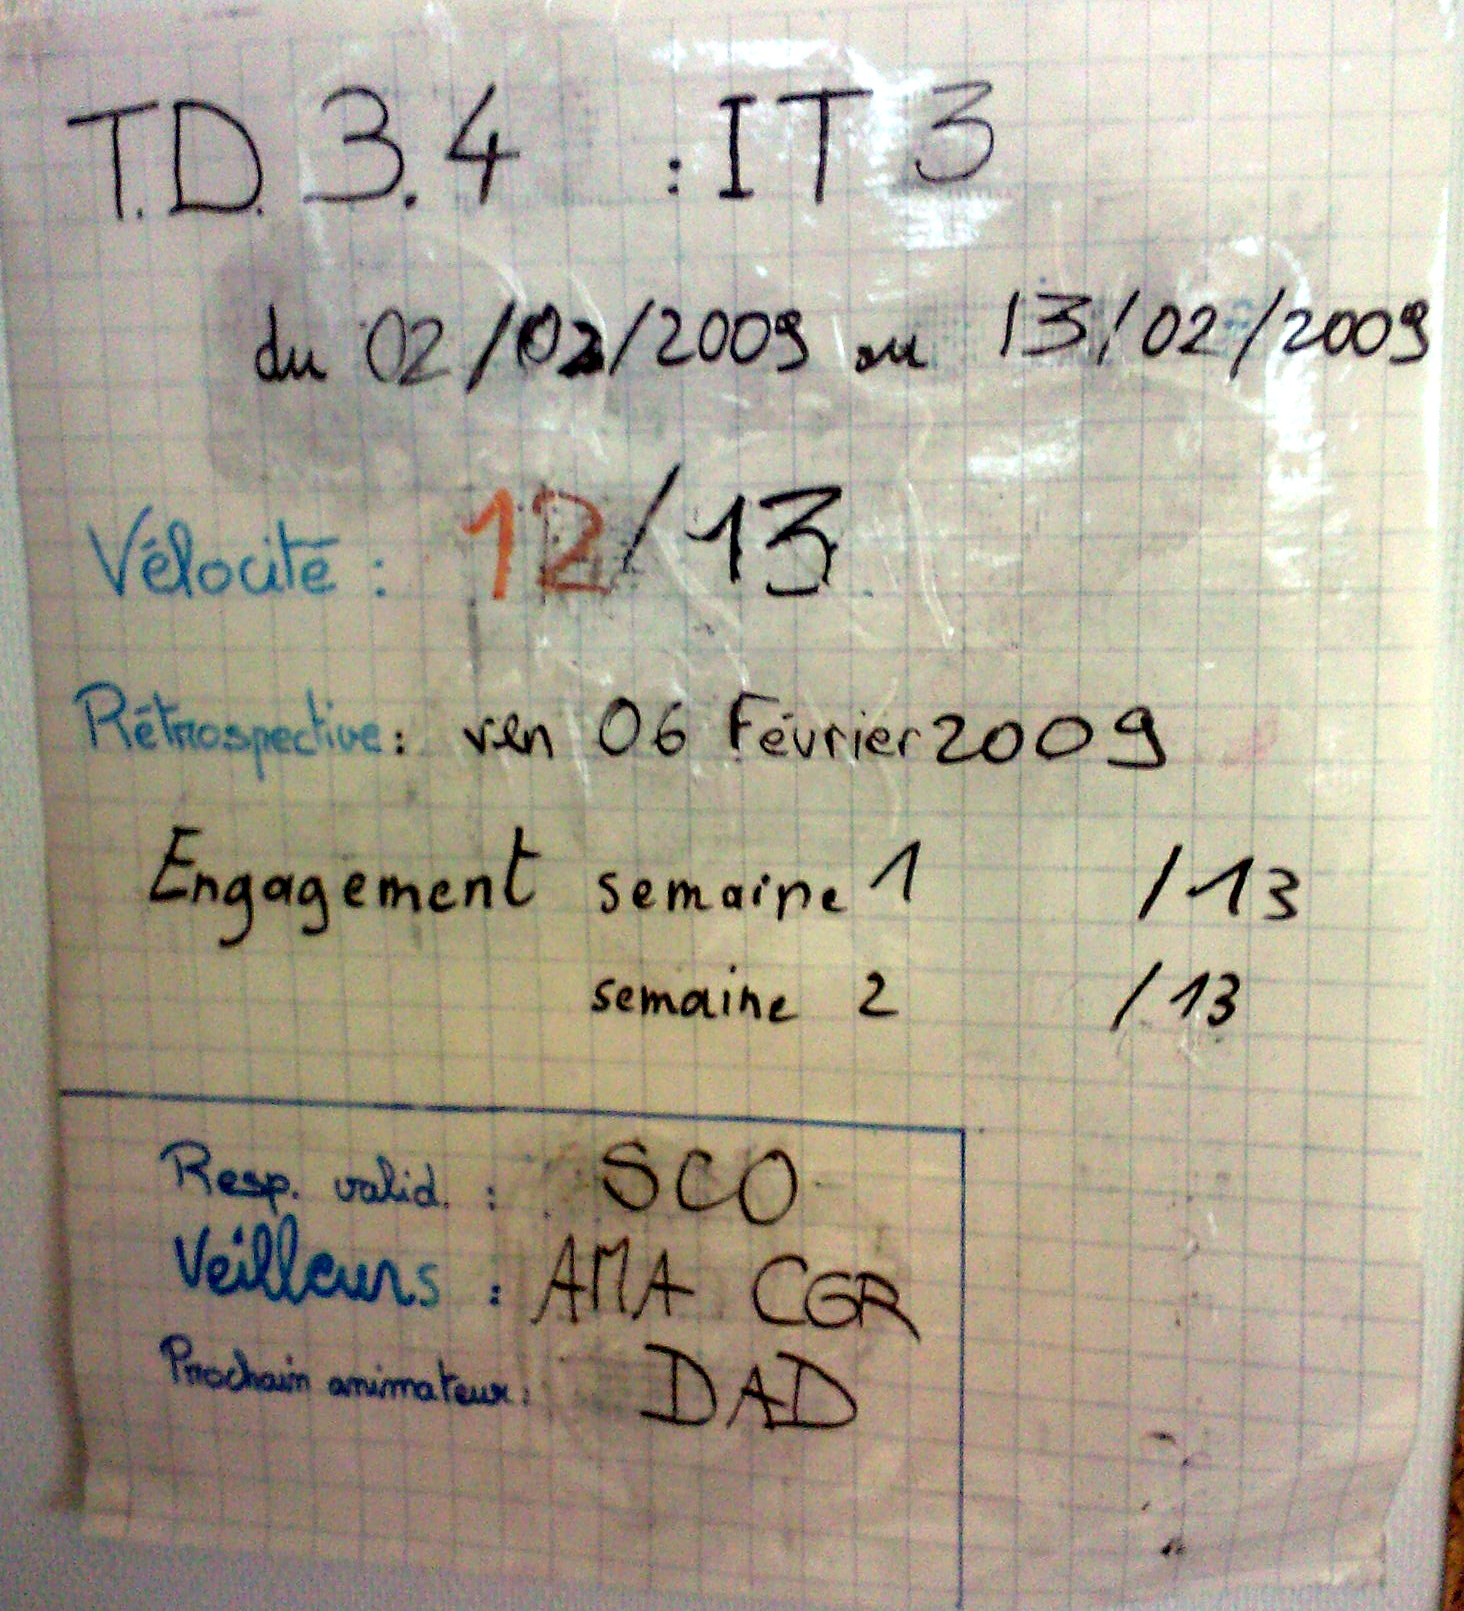
\includegraphics[scale=0.10]{Illustrations/SP_A0182.jpg}
\caption{Iteration}
\label{fig:Iteration}
\end{figure}

\subsection{Rétrospective}
Lors d'une rétrospective,  les membres de l'équipe de R\& D se réunissent pour parler de la précédente itération et pour planifier celle à venir. La réunion commence par un « check in » pendant lequel une question est posée (par exemple « Comment voyez vous Test Designer dans un an?).Un point sur des statistiques (métriques) telles que le nombre de lignes de code, le nombre de tests unitaires ou encore la vélocité atteinte par rapport aux objectifs est fait. Le point est ensuite porté sur les fonctionnalités qui ont été réalisées ou non lors de l'itération. La réunion se continue par les discussions diverses, chacun peut discuter de diverses choses : apparition de problèmes, amélioration du fonctionnement de l'équipe. La réunion se termine enfin par l'annonce de la prochaine vélocité et l'attribution des responsabilités pour l'itération qui vient. En effet chaque itération a des responsables différents (animateur de la rétrospective, validation, veilleur ...)
\subsection{Fiches}
Des fiches correspondent aux différentes t\^aches à effectuer dans le cadre d'une itération. Elles peuvent \^etre de type différent : valeur client (couleur blanche), T\^ache technique (couleur verte), Point technique (couleur bleue), Anomalie (couleur rouge), Amélioration de process (couleur jaune). Les couleurs des fiches permettent à l'équipe d'identifier au premier coup d'oeil le travail à réaliser et l'urgence. Si le tableau comporte beaucoup de fiches rouges, elles seront à traiter en priorité car ce sont des bugs. Les fiches possèdent des points qui correspondent à la quantité de travail à effectuer (en demie-journée par bin\^ome) sur la t\^ache. Si la fiche est trop importante elle peut \^etre redécoupées en fiches plus petites.

%\caption{Tux, le pingouin}
%\label{Tux}
%
%Ensuite, on s'en sert comme d'habitude (noter l'utilisation du tilde -- espace insécable -- pour garder les numéros près des mots qui les introduisent) :
%
%Dans le tableau~\ref{Tux}, page~\pageref{Tux}, nous lisons...

\begin{figure}[!h]
\centering
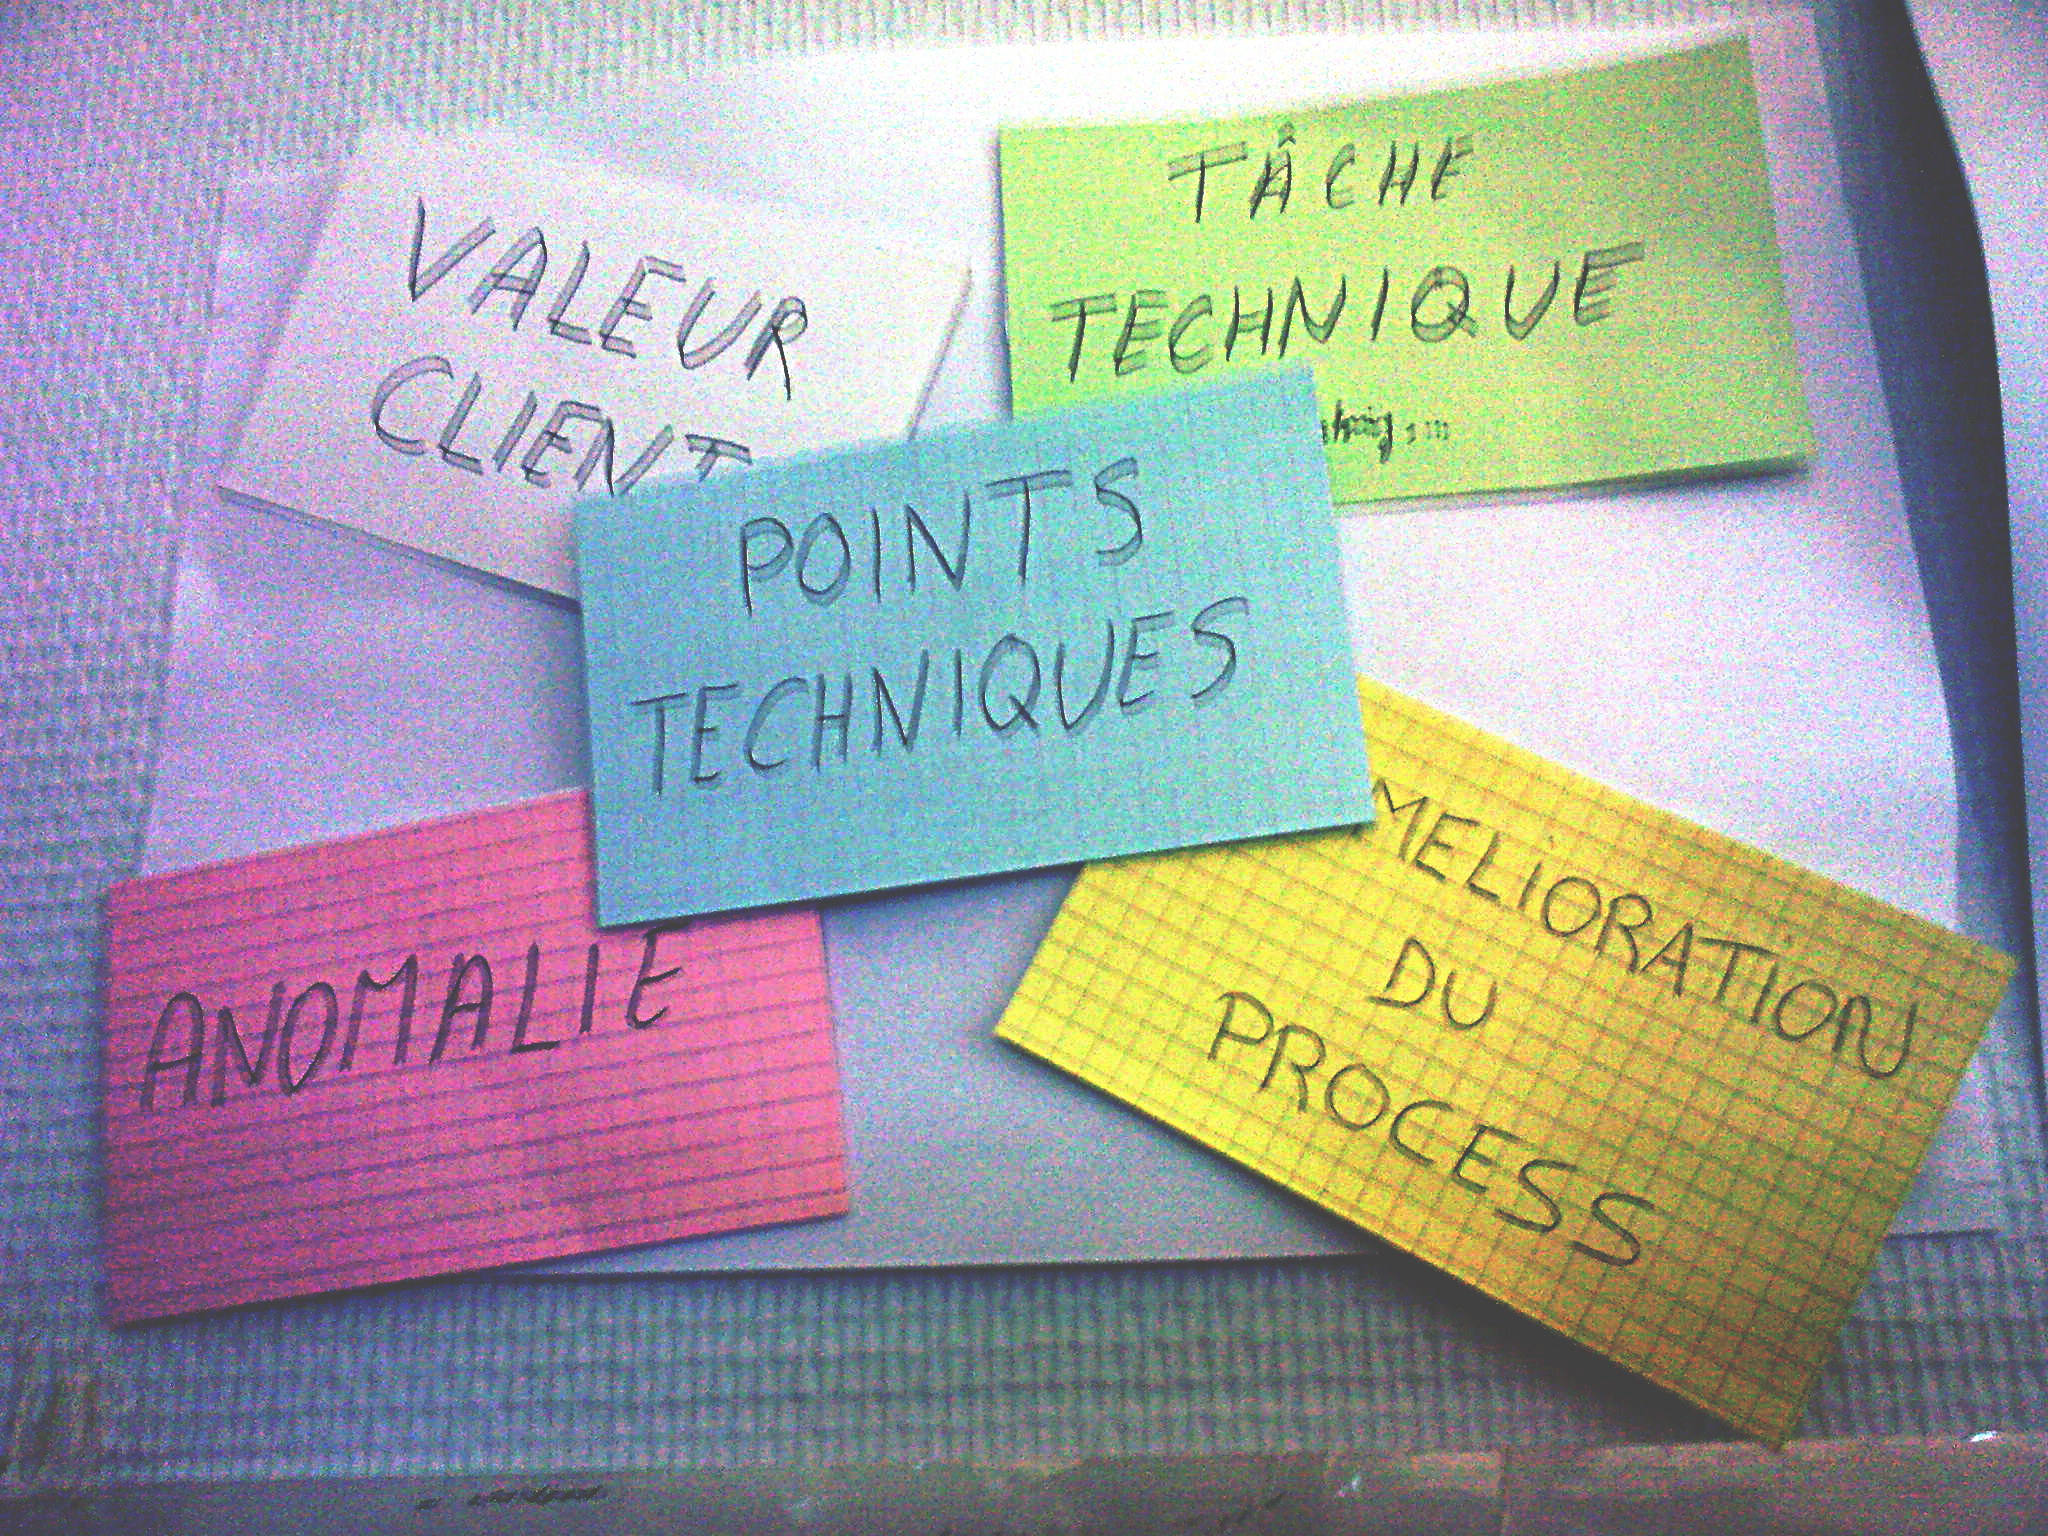
\includegraphics[scale=0.10]{Illustrations/SP_A0185.jpg}
\caption{Fiches}
\label{fig:Fiches}
\end{figure}
\begin{figure}[!h]
\centering
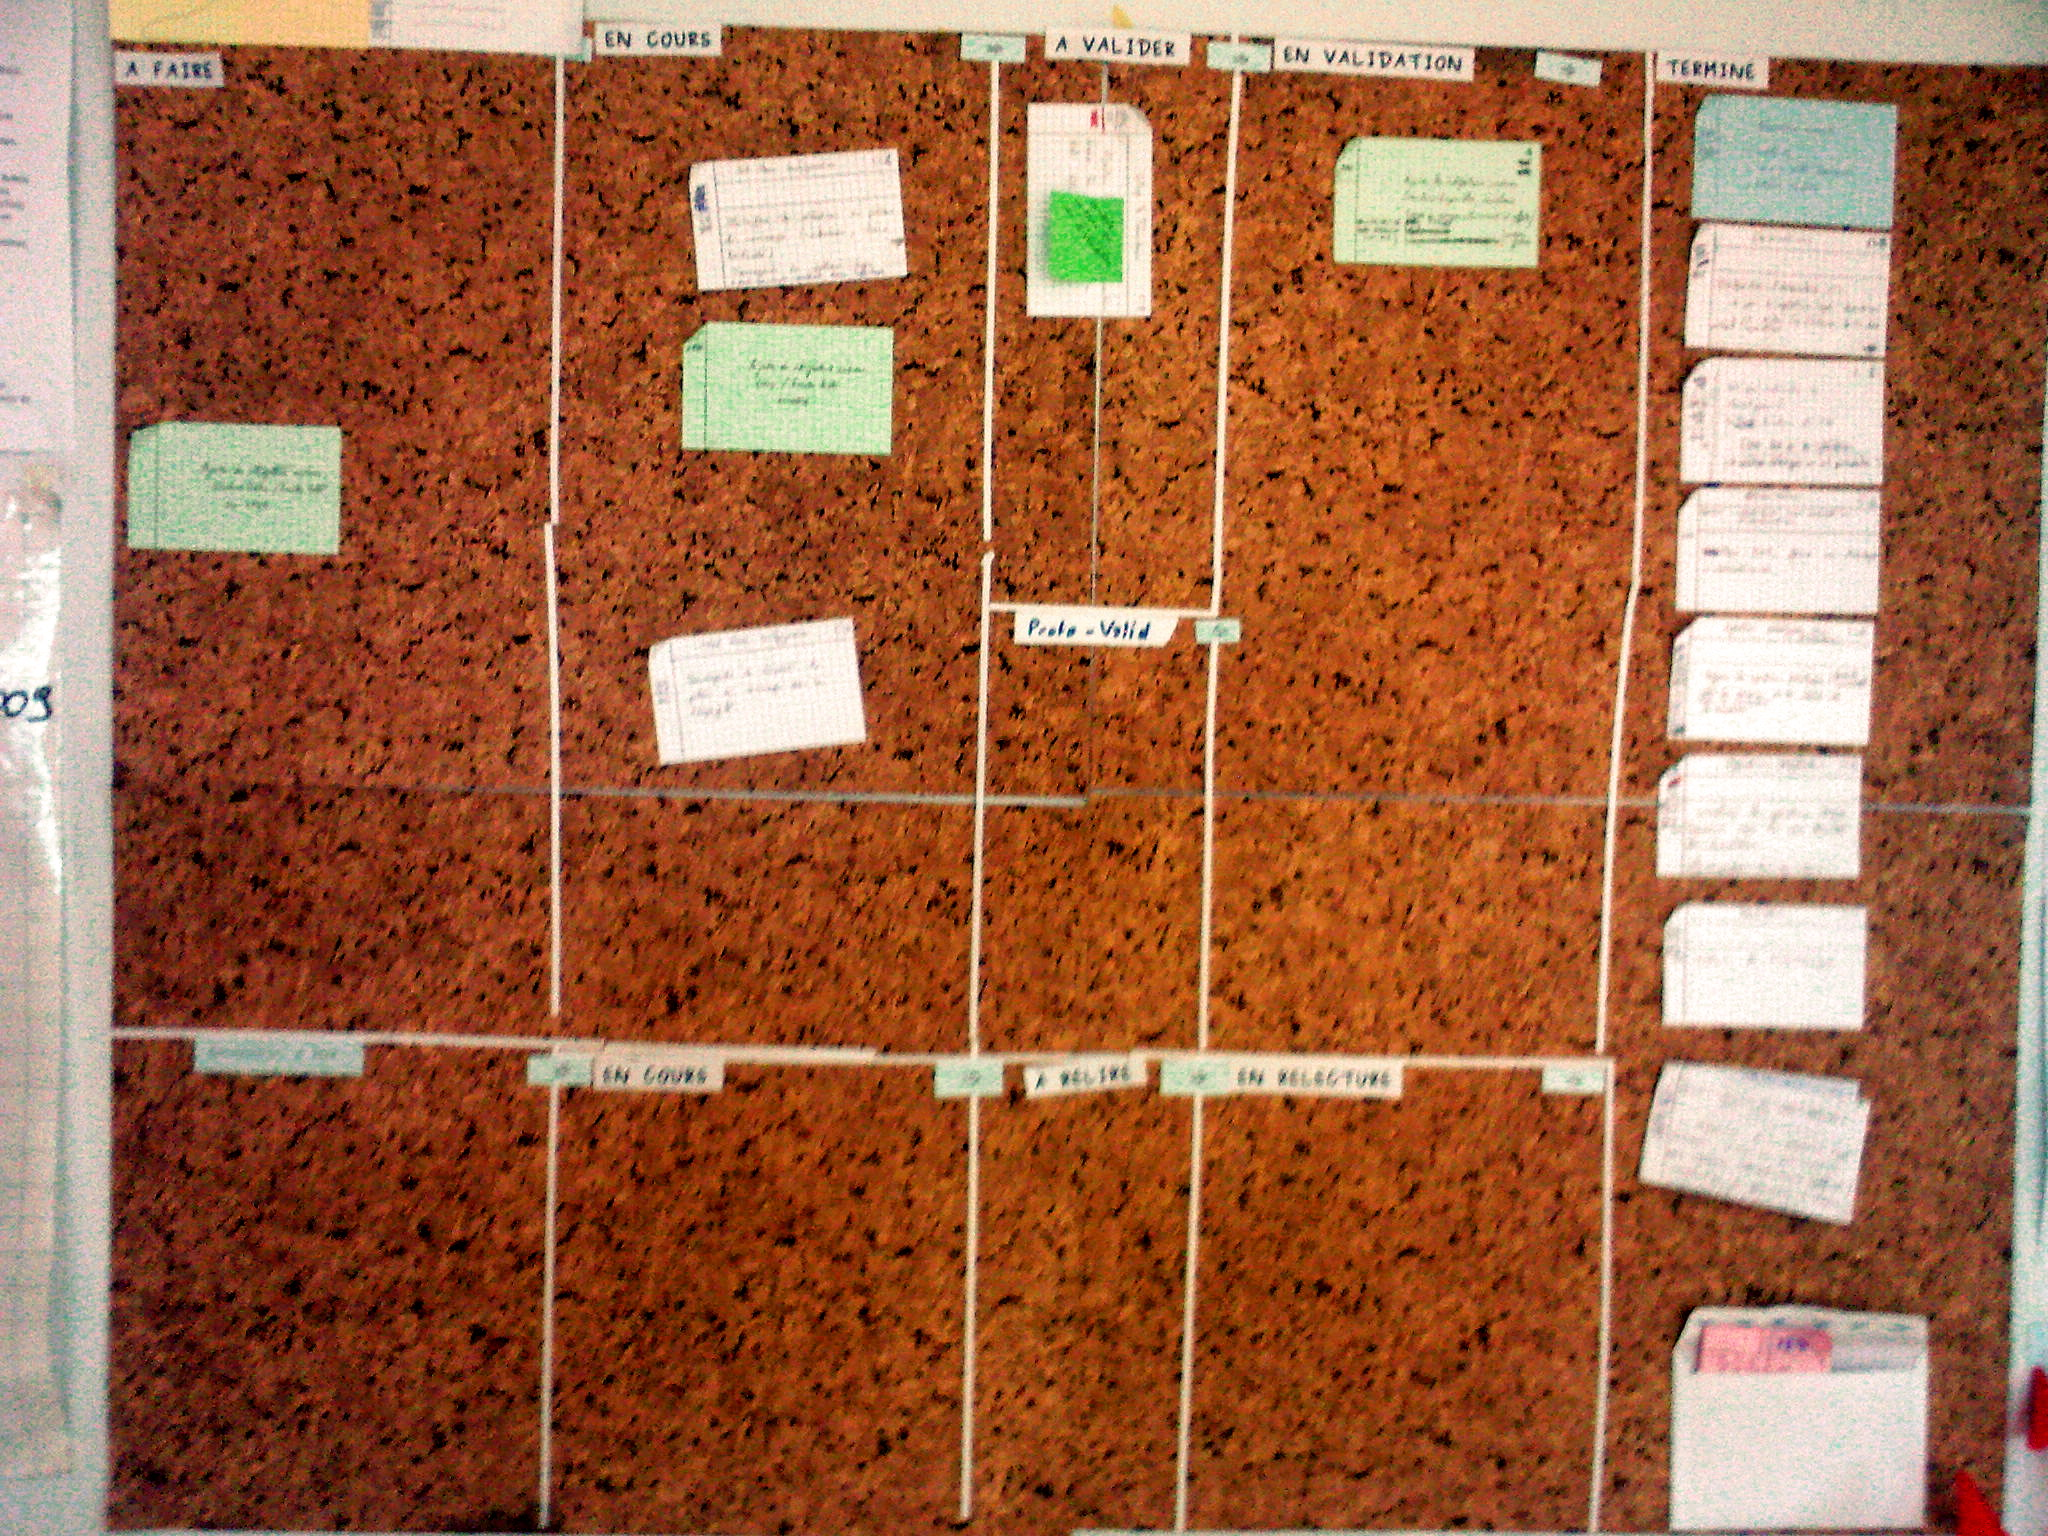
\includegraphics[scale=0.10]{Illustrations/SP_A0183.jpg}
\caption{Tableau d'avancement des fiches}
\label{fig:Tableau d'avancement des fiches}
\end{figure}
\subsection{Travail en binômes (pair programming)}
Une grand partie du travail dans l'équipe est réalisée en binôme. Les binômes changent très souvent. Les avantages du travail en binôme sont multiples. Contrairement à la programmation individuelle les binômes permettent de diffuser plus rapidement le savoir acquis lors du développement et seront plus à même à partager leur connaissances (effet boule de neige). De plus des études montrent que le travail par paires donne généralement un code de meilleure qualité, une meilleure capture des bugs. La communication et la motivation dans l'équipe sont également améliorées par cette méthode.
\begin{figure}[!h]
\centering
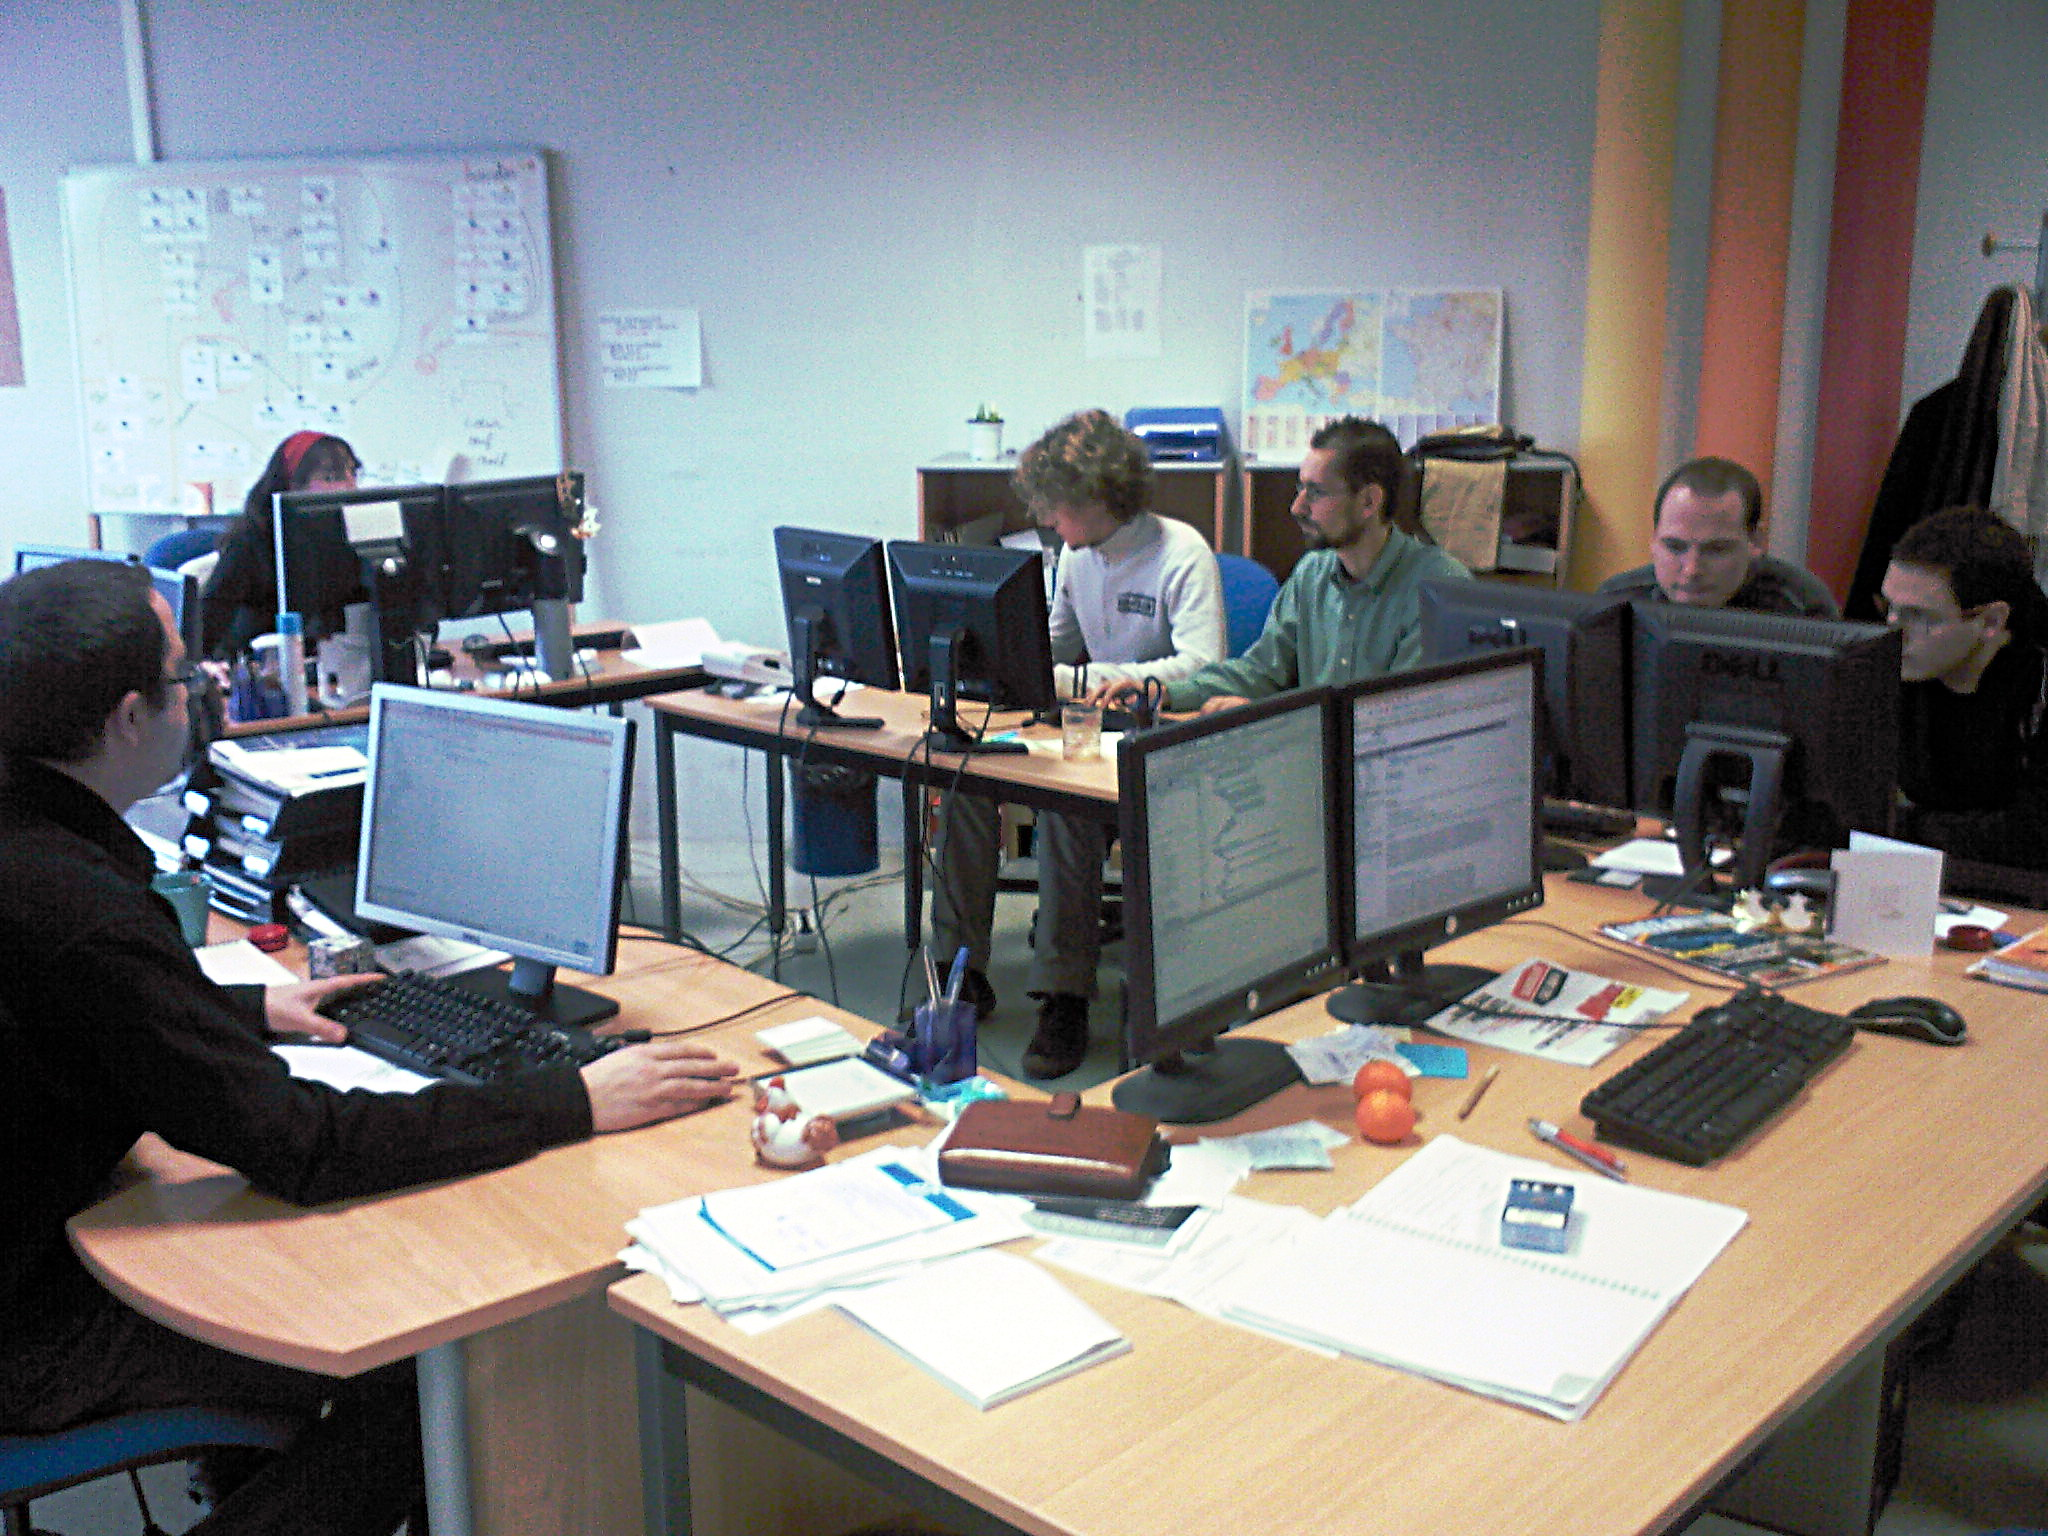
\includegraphics[scale=0.15]{Illustrations/SP_A0188.jpg}
\caption{Pair programming}
\label{fig:Pair programming}
\end{figure}
\subsection{Validation}
La validation joue un rôle important lors de l'intégration continue. Elle ne peut être réalisée que par des personnes qui n'ont pas participé au développement de la fonctionnalité. Cela permet d'avoir une idée plus objective des manipulations à effectuer pour tester la fonctionnalité. La validation es supervisée par le Client XP.


\subsection{Emploi du temps}
\subsubsection{Morning meeting}
Les membre de l'équipe se réunissent juste avant la pause déjeuner pour parler de ce qu'ils ont fait la matinée afin d'informer toute l'équipe de l'avancée de leur engagement ainsi que des problèmes qu'ils rencontrent . Toute l'équipe est réunie en cercle et se passe un objet. Celui qui a l'objet prend la parole. Le temps de parole est très bref et si un problème mérite une attention particulière il sera traité hors du cercle plus tard.

\subsubsection{Point perso}
Le mardi, juste avant la pause déjeuner, un membre de l'équipe fait une présentation à l'aide d'un projecteur sur un sujet de son choix (pas nécessairement lié à l'informatique d'ailleurs). La présentation doit durer 10 minutes. \`A la fin, les membres de l'équipe peuvent poser des questions et commenter la manière dont la présentation a été réalisée (Intéresser le public, parler clairement, qualité du support...).

\subsubsection{Discussion sur un livre}
L'équipe lit un livre pendant la semaine et se réunit le mercredi avant la pause de midi pour commenter un chapitre. L'équipe lorsque je suis arrivé lisait « The Art of Agile Development ». Cette activité permet deja de lire en anglais , mais également d'améliorer la cohésion de l'équipe par l'éventuelle adoption de pratiques nouvelles.
Point technique
Le Jeudi matin en début de matinée à lieu le point technique il peut varier dans son contenu. Cela peut aller de la discussion d'un point technique rencontré lors de l'itération à un code contest de 30 minutes.

\section{Activités confiées pendant le stage}
\subsection{Travail sur IDEA, svn, ...}
TODO : mise en place, utilisation, utilité ...
\subsection{Développement sur le code de production}
TODO : Correction bug affichage no changes, travail sur Setup/teardown, 
\subsection{Documentation}

\subsection{Validation}
La validation des fiches est obligatoire pour considérer que la fonctionnalité lui correspondant est terminée. Elle consiste au test de la fonctionnalité sur l'application après commit. La validation se fait généralement en binôme et il faut chercher toutes les combinaisons en rapport avec la nouvelle fonctionnalité qui sont susceptible d'échouer, de vérifier si toutes les objectifs de la fiche sont remplis. Après avoir testé un maximum de cas de figures il faut faire appel au Client XP qui va s'assurer que l'engagement a été rempli. Une fois cela fait, la fiche est terminée et son nombre de points de vélocité peut être ajouté à ce qui a déjà été fait
\subsection{Amélioration du code existant (refactoring)}
TODO : utilité ,exemple, 
\subsection{Administration système}
Sur une courte période j'ai effectué des t\^aches d'administration système. En particulier au moment de l'intégration des Google Apps dans le fonctionnement de Smartesting. La necessité de partager des calendriers et de pouvoir y accéder via des plateformes mobiles a amené Smartesting à envisager d'utiliser Google Apps. Ainsi, en binôme avec Olivier, nous avons appréhendé le panneau d'administration ainsi que les différents services utilisables. Chaque calendrier donne la possibilité d'être exporté, ainsi nous avons pu réaliser une routine de backup\footnote{sauvegarde automatique}.
\subsection{Meeting corporate}
TODO : definition, utilité, ma participation ...
\subsection{Visite de BNP Paribas}
Mes impressions, les decisions, Smart et BNP ...

\subsection{Amélioration du process, évolution du fonctionnement de l'équipe}
J'ai été ammené à l'occasion de retrospectives ou de réunions à réfléchir sur le processus de développement au sein de l'équipe. L'équipe de R\&D est très concernée par l'amélioration du processus et toute pratique peut être remise en cause si elle ne convient pas a l'équipe. Chaque décision quelle qu'elle soit doit être approuvée par toute l'équipe avant d'être prise. Je parlerai plus en détail à travers d'exemple du type de décisions qui sont prises sur ce sujet.
TODO : Pomodoro, Decisions lors de retrospectives, Iteration 1 semaine, Slack, reduction de vélocité, Done-done, rédaction(et simplification) des standards, Objectifs R\& D, ...

\subsection{Connaissances acquises}
Programmation JAVA
Utilisation de tests unitaires.
Design patterns
Travail en Open-Space
Initiation à la méthode Agile en particulier à l'eXtreme Programming

\subsection{Apport à l'entreprise d'accueil}

\section{Conclusion}

\section{Lexique}
\paragraph{Technologie JAVA}
JAVA est le nom d'une technologie mise au point par Sun Microsystems qui permet de produire des logiciels indépendants de toute architecture matérielle. Cette technologie s'appuie sur différents éléments qui, par abus de langage, sont souvent tous appelés Java.
\paragraph{Langage JAVA}
Le Langage Java est un langage de programmation informatique orienté objet créé par James Gosling et Patrick Naughton employés de Sun Microsystems avec le soutien de Bill Joy (cofondateur de Sun Microsystems en 1982), présenté officiellement le 23 mai 1995 au SunWorld. Le langage Java a la particularité principale que les logiciels écrits avec ce dernier sont très facilement portables sur plusieurs systèmes d'exploitation tels que Unix, Microsoft Windows, Mac OS ou Linux avec peu ou pas de modification... C'est la plate-forme qui garantit la portabilité des applications développées en Java. Le langage reprend en grande partie la syntaxe du langage C++, très utilisé par les informaticiens. Néanmoins, Java a été épuré des concepts les plus subtils du C++ et à la fois les plus déroutants, tels que l'héritage multiple 	 l'embauche par Jim Blandy de Karl Fogel, qui travaillait déjà sur un nouveau gestionnaire de version. 

\paragraph{Agile}
Les méthodes Agiles sont des procédures de conception de logiciel qui se veulent plus pragmatiques que les méthodes traditionnelles. En impliquant au maximum le demandeur (client), ces méthodes permettent une grande réactivité à ses demandes, visent la satisfaction réelle du besoin du client, et non des termes du contrat de développement. La notion de méthode agile est née à travers un Manifeste Agile signé par 17 personnalités. La notion de méthode agile se limite actuellement aux méthodes ciblant le développement d'une application informatique.

\paragraph{XP}
L'Extreme Programming (XP) est une méthode agile de gestion de projet informatique adaptée aux équipes réduites avec des besoins changeants. Elle pousse à l'extrême des principes simples. 

\paragraph{Vélocité}
Système permettant de mesurer l'avancée du projet en attribuant des points de vélocité aux fiches (tâches) validées par les développeurs.

\paragraph{Itération}
L'équipe de réalisation s'engage sur sur ce qui va être livré. Une itération a en général une durée de 1 à 2 semaines. Une itération se termine par la livraison des nouvelles fonctionnalités et une rétrospective qui planifie l'itération suivante.

\paragraph{Intégration continue}
Lorsqu'une tâche est terminée, les modifications sont immédiatement intégrées dans le produit complet. On évite ainsi la surcharge de travail liée à l'intégration de tous les éléments avant la livraison. Les tests facilitent grandement cette intégration : quand tous les tests passent, l'intégration est terminée. 
Programmation en bin\^ome : La programmation se fait par deux. Le premier appelé driver (ou pilote) tient le clavier. C'est lui qui va travailler sur la portion de code à écrire. Le second appelé partner (ou co-pilote) est là pour l'aider en suggérant de nouvelles possibilités ou en décelant d'éventuels problèmes. Les développeurs changent fréquemment de partenaire ce qui permet d'améliorer la connaissance collective de l'application et d'améliorer la communication au sein de l'équipe. 

\paragraph{Tests unitaires}
En programmation informatique, le test unitaire est un procédé permettant de s'assurer du fonctionnement correct d'une partie déterminée d'un logiciel ou d'une portion d'un programme (appelée « unité »).
Il s'agit pour le programmeur de tester un module, indépendamment du reste du programme, ceci afin de s'assurer qu'il répond aux spécifications fonctionnelles et qu'il fonctionne correctement en toutes circonstances. Cette vérification est considérée comme essentielle, en particulier dans les applications critiques. Elle s'accompagne couramment d'une vérification de la couverture de code, qui consiste à s'assurer que le test conduit à exécuter l'ensemble (ou une fraction déterminée) des instructions présentes dans le code à tester.
L'ensemble des tests unitaires doit être rejoué après une modification du code afin de vérifier qu'il n'y a pas de régressions (l'apparition de nouveaux dysfonctionnements).
Dans les applications non critiques, l'écriture des tests unitaires a longtemps été considérée comme une tâche secondaire. Cependant, la méthode Extreme programming (XP) a remis les tests unitaires, appelés « tests du programmeur », au centre de l'activité de programmation.
La méthode XP préconise d'écrire les tests en même temps, ou même avant la fonction à tester (Test Driven Development). Ceci permet de définir précisément l'interface du module à développer. En cas de découverte d'un bogue, on écrit la procédure de test qui reproduit le bogue. Après correction on relance le test, qui ne doit indiquer aucune erreur.
\paragraph{Tests haut niveau}
\paragraph{MBT}
Parmi les différentes approches du test logiciel, MBT (Model Based Testing) a pour objectif de créer des cas de test à partir de modèles abstraits.
\paragraph{Tests fonctionnels}
À partir des scénarios définis par le client, l'équipe crée des procédures de test qui permettent de vérifier l'avancement du développement. Lorsque tous les tests fonctionnels passent, l'itération est terminée. Ces tests sont souvent automatisés mais ce n'est pas toujours possible.
\paragraph{Refactoring}
La refactorisation (anglicisme venant de refactoring) est une opération de maintenance du code informatique. Elle consiste à retravailler le code source non pas pour ajouter une fonctionnalité supplémentaire au logiciel mais pour améliorer sa lisibilité, simplifier sa maintenance, ou changer sa généricité (on parle aussi de remaniement). Une traduction plus appropriée serait réusinage. C'est donc une technique qui s'approche de l'optimisation du code, même si les objectifs sont radicalement différents. 
\paragraph{IntelliJ IDEA}
IntelliJ IDEA est un environnement de développement JAVA qui permet entre autres la refactorisation de code.
\paragraph{Client XP}
Appelé également client sur site; 
\paragraph{Commit}
\paragraph{Code contest}
\section{Bibliographie}
- Wikipedia : 
http://fr.wikipedia.org
http://en.wikipédia.org
